% Author: Kjell Magne Fauske
% Source: http://www.texample.net/tikz/examples/prims-algorithm/
% Declare layers
\pgfdeclarelayer{background}
\pgfsetlayers{background,main}

\subsection{Algorithmus von Prim}
\begin{frame}{Algorithmus von Prim}{Prim's algorithm}
	$S$ ist Menge aller erreichten Knoten, $E$ ist Menge der ausgewählten Kanten.\pause



	Starte bei einem beliebigen Knoten: füge zu $S$ hinzu.
	\begin{enumerate}
		\item wähle Kante am \emph{Rand} von $S$ mit dem geringsten Gewicht und füge zu $E$ hinzu. \pause
		\item füge zugehörigen Knoten zu $S$ hinzu.
		\item Fehlt ein Knoten in $S$ ? goto 1
	\end{enumerate}
\end{frame}

\begin{frame}{Algorithmus von Prim}{Prim's algorithm}
	%% Adjacency matrix of graph
	%% \  a  b  c  d  e  f  g
	%% a  x  7     5
	%% b  7  x  8  9  7
	%% c     8  x     5
	%% d  5  9     x 15  6
	%% e     7  5 15  x  8  9
	%% f           6  8  x 11
	%% g              9  11 x
	\begin{figure}
		\begin{tikzpicture}[scale=1.8, auto,swap]
			% Draw a 7,11 network
			% First we draw the vertices
			\foreach \pos/\name in {{(0,2)/a}, {(2,1)/b}, {(4,1)/c},
				                    {(0,0)/d}, {(3,0)/e}, {(2,-1)/f}, {(4,-1)/g}}
				\node[vertex] (\name) at \pos {$\name$};
			% Connect vertices with edges and draw weights
			\foreach \source/ \dest /\weight in {b/a/7, c/b/8,d/a/5,d/b/9,
				                                 e/b/7, e/c/5,e/d/15,
				                                 f/d/6,f/e/8,
				                                 g/e/9,g/f/11}
				\path[edge] (\source) -- node[weight] {$\weight$} (\dest);
			% Start animating the vertex and edge selection.
			\foreach \vertex / \fr in {d/1,a/2,f/3,b/4,e/5,c/6,g/7}
				\path<\fr-> node[selected vertex] at (\vertex) {$\vertex$};
			% For convenience we use a background layer to highlight edges
			% This way we don't have to worry about the highlighting covering
			% weight labels.
			\begin{pgfonlayer}{background}
				\pause
				\foreach \source / \dest in {d/a,d/f,a/b,b/e,e/c,e/g}
				    \path<+->[selected edge] (\source.center) -- (\dest.center);
				\foreach \source / \dest / \fr in {d/b/4,d/e/5,e/f/5,b/c/6,f/g/7}
				    \path<\fr->[ignored edge] (\source.center) -- (\dest.center);
			\end{pgfonlayer}
		\end{tikzpicture}
	\end{figure}
\end{frame}
%% end of source

\begin{frame}{Algorithmus von Prim}{Prim's algorithm}
%source http://inserv.math.muni.cz/biografie/obrazky/jarnik_vojtech.jpg
%http://www.ams.org/featurecolumn/images/january2006/trees9.jpg
	\textbf{Erfinder}
	\begin{itemize}
		\item 1930: Vojtěch Jarník
		\item 1957: Robert C. Prim
		\item 1959 wiederentdeckt von Edsger Dijkstra
	\end{itemize}

	\begin{figure}
\centering
\mbox{\subfigure{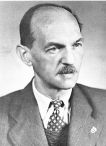
\includegraphics[width=0.6in]{Material/jarnik_vojtech.jpg}}\quad
\subfigure{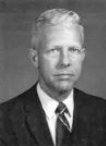
\includegraphics[width=0.6in]{Material/Prim.jpg} }}
\caption{Jarnik Vojtech und Prim}
\end{figure}
	\textbf{Alternative Bezeichnungen}
	\begin{itemize}
		\item DJP algorithm
		\item Jarník algorithm
		\item Prim–Jarník algorithm
	\end{itemize}

\end{frame}